\chapter{Platform adaptivity}

\chapterintro{This chapter introduces concepts and mechanisms that enhance a platform with adaptivity capabilities, which are often achieved by fusion of rules, policies and scaling techniques.}

\section{Introduction}
In short, platform adaptivity adds a auto-scaling features to a solution offered by Platform-as-a-Service provider. Key concept is to have a Elasticity Controller which gathers probes from virtual machines and uses that knowledge to execute appropriate action on cloud instance, indirectly modifying consecutive probes \cite{VaRoBu11}. This concept illustrates diagram \ref{ch3:elasticity-controller}.

\begin{figure}[!ht]
  \begin{center}
    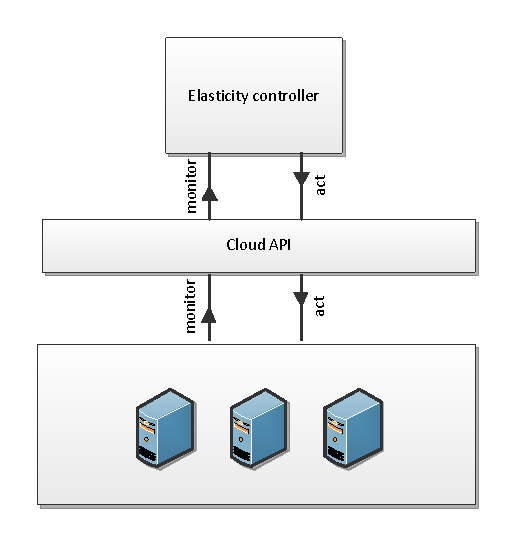
\includegraphics{chapter-3/elasticity-controller}
  \end{center}
  \caption{Elasticity controller}
  \label{ch3:elasticity-controller}
\end{figure}

The remaining of this chapter describes crucial elements that compose elasticity controller: policies, data analysis, triggered actions and presents a comparison of cloud providers.
 
\section{Policies}
While auto-scaling is offered by a vast amount of cloud providers (e.g AWS, OpenShift, OpenNebula) it often lacks a sophisticated mechanisms allowing for specific scaling policies, being limited to only one predefined rule as it is in case of OpenShift for example. 
 
Policy denotes a condition which, when satisfied, triggers an action that is supposed to harness cloud instance in a way that future evaluations of condition will be unsuccessful. Typically condition itself is accompanied by a minimal and maximal number of node instances, allowing for ensuring minimal QoS and controlling maximal costs. Currently, industry leaders supports two main kind of policies \cite{AmazonAutoScaling}:
\begin{itemize}
 \item \textit{expression based} - allows to define how you to scale application in response to changing conditions, which include factors such as memory, CPU usage, cost or some indirect, calculated metrics
 \item \textit{scheduled} - allows to scale an application in response to predictable load changes. For example, traffic increases during the weekends and decreases on working days. Hence, that predictable traffic patterns is used to scale application based on current time.
\end{itemize}

Technically, policies are expressed in some human-readable format such as JSON, XML as it is in case of AWS EC2 or custom expression used for example by Carina. Appendix \ref{app:scaling-policies} presents example configuration used by AWS E2 Auto-Scaling.

\section{Data analysis}
Having policies defined, their conditions are evaluated against data acquired from sensors. In a simplest case this evaluation can be based on a Threshold Model \cite{LiWoZh05}, which defines a valid range. In cases when given metric violates that condition (i.e. value is either smaller than minimal or bigger than maximal acceptable) corresponding resource is properly adjusted - figure \ref{ch3:threshold-model} illustrates that idea.

\begin{figure}[!ht]
  \begin{center}
    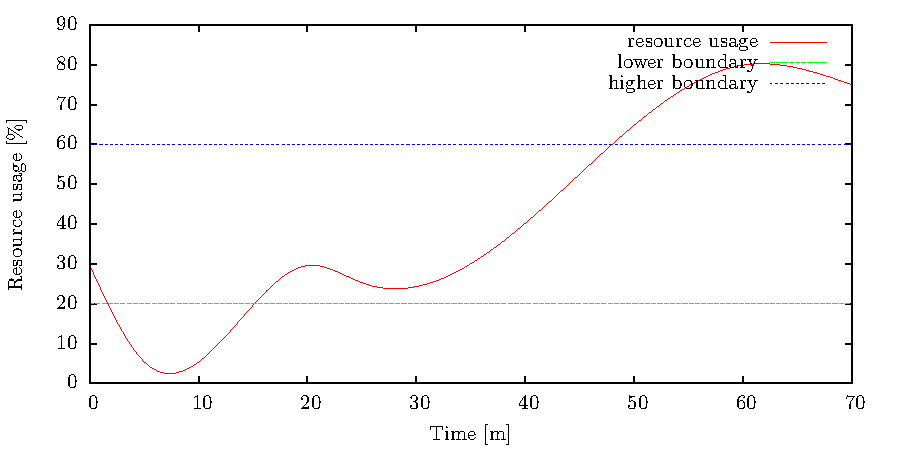
\includegraphics{chapter-3/threshold-model}
  \end{center}
  \caption{Threshold model}
  \label{ch3:threshold-model}
\end{figure}

While trivial in its form, cases of AWS, OpenShift, Carina, OneCloud proves it is useful in a real-world scenarios. Having that said, more sophisticated algorithms also exists:
\begin{itemize}
  \item \textit{integer programming} - auto scaling is reduced to server integer programming problems, which aims to minimize the cost or maximize the computing power with either computing power constraints or
budget constraints \cite{MaLiHu10}
  \item \textit{burst based padding} - employs a signal processing technique based on fast Fourier transform, burst pattern is extracted and used to calculate a padding value. Coefficients that represents the amplitude of each frequency component are used to calculate burst density. Depending of that value (i.e. is higher than 50\%) appropriate percentile of the burst values are used \cite{ShSuGuWi11}  
  \item \textit{remedial padding} - padding errors are being recorded and used in successive padding evaluations. In other words, let $e_1, e_2, ... e_k$ denote the recent prediction errors, next the weighted moving average is calculated. Actual applied padding is either padding itself or weighted average, depending which one is greater \cite{ShSuGuWi11}    
  \item \textit{linearised dynamic control} - linearised correction model is based on control equations \cite{AbShBh02}:
  
    \begin{equation}
      x(k+1)=Ax(k)+Bu(k)
    \end{equation}
    
    \begin{equation}
       y(k) = C x(k) + D u(k) + E z(k)
    \end{equation}
    where x denotes the state variable vector and coefficient matrices: A B C D E are fitted to historical data as a regression model - \cite{DiLuFrHePa03}

  \item \textit{markov decision process model} - computes optimal reaction to state changes by using observation on the system with assumptions about the rate of changes expected in the future \cite{AbWo02}
\end{itemize}

\section{Triggered actions}
Actions that are being triggered by a elasticity controller are focused on application scaling. Previous chapter described that problem in detail.

\section{Providers comparison}

Table \ref{tab:cloud-providers-adaptivity} summaries chapter with approaches to adaptivity taken by different cloud providers. Section 'triggered action' is omitted for brevity - it was described extensively in previous chapter.

\begin{table}[!htbp]
\begin{tabularx}{\textwidth}[]{ X  X X }
\specialrule{.1em}{.05em}{.05em} 

  & \textbf{Policies} & \textbf{Data analysis} \\
\specialrule{.1em}{.05em}{.05em} 

\multicolumn{3}{ l }{\textbf{Infrastructure provider}} \\
\specialrule{.1em}{.05em}{.05em} 

Carina & 
-- time frame based

-- expression based (only for CPU)
&
-- threshold model that takes into account minimal and maximal permitted instances of an application as well as application priority

\\ \hline

OneFlow 4.2 & 
-- time frame based with customizable padding 

-- expression based build on custom language, where all vm's metrics are supported

-- customizable adjustment padding, cooldown time
&
-- threshold model

\\ \hline

AWS EC2 & 
-- time frame based

-- expression based, where expressions corresponds to a AutoScalingGroup

-- actions are triggered by a CloudWatch alarms

-- customizable adjustments paddings, types, cooldown time
&
-- threshold model, takes into account minimal and maximal permitted instances of an application as well as application priority
\\ \hline

\multicolumn{3}{ l }{\textbf{Platform provider}} \\
\specialrule{.1em}{.05em}{.05em} 

CloudFoundry & $\times$ & $\times$ \\ \hline

OpenShift & 
-- single built-in policy

 &
-- single built-in threshold model that scales an application when CPU load is greater than 50\% for a given period
\\ \hline

AppEngine & 

-- built-in policy based on request queue length

-- adjustable minimal, maximal number of application instances, pending latency

 &
-- queue-based, new instance is provisioned if queue length got too long 
  \\ \hline

Azure & 
-- time frame based

-- expression based, where expression can involve either CPU usage or Queue length

-- customizable adjustments paddings, types, cooldown time
&
-- threshold model, that takes into account minimal and maximal allowed instances
 \\ \hline

Heroku & $\times$ & $\times$ \\ \hline
\end{tabularx}

\caption{Comparison of cloud providers approach to adaptivity}
\label{tab:cloud-providers-adaptivity}

\end{table}

